%\documentclass[12pt,a4paper]{scrartcl}
\documentclass[12pt,a4paper]{article}

\makeatletter % Technical doc - START

% ---------------------- %
% -- GENERAL SETTINGS -- %
% ---------------------- %

\usepackage[
	top    = 2cm,
	bottom = 2cm,
	left   = 1.5cm,
	right  = 1.5cm
]{geometry}

\usepackage[utf8]{inputenc}
\usepackage[T1]{fontenc}
\usepackage{ucs}

\usepackage[french]{babel,varioref}

\usepackage{color}
\usepackage{hyperref}
\hypersetup{
    colorlinks,
    citecolor = black,
    filecolor = black,
    linkcolor = black,
    urlcolor  = black
}
\usepackage[numbered]{bookmark}

\usepackage{enumitem}
\usepackage{multicol}
\usepackage{longtable}
\usepackage{makecell}

\setlength{\parindent}{0cm}
\setlist{noitemsep}



% --------------- %
% -- TOC & Co. -- %
% --------------- %

\usepackage[raggedright]{titlesec}

%\renewcommand\thechapter{\Alph{chapter}.}
\renewcommand\thesection{\Roman{section}.}
\renewcommand\thesubsection{\arabic{subsection}.}
\renewcommand\thesubsubsection{\roman{subsubsection}.}


\titleformat{\paragraph}[hang]{\normalfont\normalsize\bfseries}{\theparagraph}{1em}{}
\titlespacing*{\paragraph}{0pt}{3.25ex plus 1ex minus .2ex}{0.5em}


% Source
%    * https://tex.stackexchange.com/a/558025/6880
\usepackage{tocbasic}[2020/07/22]% needs KOMA-Script version 3.31

\DeclareTOCStyleEntries[
    raggedentrytext,
    linefill = \hfill,
    indent   = 0pt,
    dynindent,
    numwidth = 0pt,
    numsep   = 1ex,
    dynnumwidth
]{tocline}{
	chapter,
	section,
	subsection,
	subsubsection,
	paragraph,
	subparagraph
}

\DeclareTOCStyleEntry[indentfollows = chapter]{tocline}{section}



% ----------- %
% -- TOOLS -- %
% ----------- %

\usepackage{ifplatform}
\usepackage{ifthen}
\usepackage{macroenvsign}
\usepackage{pgffor}



% ------------------------- %
% -- SPECIAL FORMATTINGS -- %
% ------------------------- %

\usepackage{amsthm}

\usepackage{tcolorbox}


% -- LISTINGS -- %

%\tcbuselibrary{listingsutf8}
\tcbuselibrary{minted, breakable}

\newtcblisting{latexex}{%
    breakable,%
    sharp corners,%
    left   = 1mm, right = 1mm,%
    bottom = 1mm, top   = 1mm,%
    %colupper = red!75!blue,%
    listing side text
}

\newtcbinputlisting{\inputlatexex}[2][]{%
    listing file={#2},%
    breakable,
    sharp corners,%
    left   = 1mm, right = 1mm,%
    bottom = 1mm, top   = 1mm,%
    %colupper = red!75!blue,%
    listing side text
}


\newtcblisting{latexex-flat}{%
    breakable,
    sharp corners,%
    left   = 1mm, right = 1mm,%
    bottom = 1mm, top   = 1mm,%
    %colupper = red!75!blue,%
}

\newtcbinputlisting{\inputlatexexflat}[2][]{%
    listing file={#2},%
    breakable,
    sharp corners,%
    left   = 1mm, right = 1mm,%
    bottom = 1mm, top   = 1mm,%
    %colupper = red!75!blue,%
}


\newtcblisting{latexex-alone}{%
    breakable,
    sharp corners,%
    left   = 1mm, right = 1mm,%
    bottom = 1mm, top   = 1mm,%
    %colupper = red!75!blue,%
    listing only
}

\newtcbinputlisting{\inputlatexexalone}[2][]{%
    listing file={#2},%
    breakable,
    sharp corners,%
    left   = 1mm, right = 1mm,%
    bottom = 1mm, top   = 1mm,%
    %colupper = red!75!blue,%
    listing only
}


\newcommand\inputlatexexcodeafter[1]{%
    \begin{center}
        \input{#1}
    \end{center}

    \vspace{-.5em}
    
    Le rendu précédent a été obtenu via le code suivant.
    
    \inputlatexexalone{#1}
}


\newcommand\inputlatexexcodebefore[1]{%
    \inputlatexexalone{#1}
    \vspace{-.75em}
    \begin{center}
        \textit{\footnotesize Rendu du code précédent}
        
        \medskip
        
        \input{#1}
    \end{center}
}


% -- REMARK -- %

\theoremstyle{definition}
\newtheorem*{remark}{Remarque}


% -- EXAMPLE -- %

\newcounter{paraexample}[subsubsection]

\newcommand\@newexample@abstract[2]{%
    \paragraph{%
        #1%
        \if\relax\detokenize{#2}\relax\else {} -- #2\fi%
    }%
}

\newcommand\newparaexample{\@ifstar{\@newparaexample@star}{\@newparaexample@no@star}}

\newcommand\@newparaexample@no@star[1]{%
    \refstepcounter{paraexample}%
    \@newexample@abstract{Exemple \theparaexample}{#1}%
}

\newcommand\@newparaexample@star[1]{%
    \@newexample@abstract{Exemple}{#1}%
}


% -- CHANGE LOG -- %

\newcommand\topic{\@ifstar{\@topic@star}{\@topic@no@star}}

\newcommand\@topic@no@star[1]{%
    \textbf{\textsc{#1}.}%
}

\newcommand\@topic@star[1]{%
    \textbf{\textsc{#1} :}%
}


% -- ABOUT MACROS & Co. -- %

\newcommand\env[1]{\texttt{#1}}
\newcommand\macro[1]{\env{\textbackslash{}#1}}

\newcommand\separation{
    \medskip
    \hfill\rule{0.5\textwidth}{0.75pt}\hfill
    \medskip
}


\newcommand\extraspace{
    \vspace{0.25em}
}


\newcommand\whyprefix[2]{%
    \textbf{\prefix{#1}}-#2%
}

\newcommand\mwhyprefix[2]{%
    \texttt{#1 = #1-#2}%
}

\newcommand\prefix[1]{%
    \texttt{#1}%
}


\newcommand\inenglish{\@ifstar{\@inenglish@star}{\@inenglish@no@star}}

\newcommand\@inenglish@star[1]{%
    \emph{\og #1 \fg}%
}

\newcommand\@inenglish@no@star[1]{%
    \@inenglish@star{#1} en anglais%
}


\newcommand\ascii{\texttt{ASCII}}

\makeatother % Technical doc - END


\usepackage{ tnspverb }


\begin{document}

\renewcommand\labelitemi{\raisebox{0.125em}{\tiny\textbullet}}
\renewcommand{\labelitemii}{---}

\title{   %
	Le package \texttt{ tnspverb }\\%
	{\footnotesize Code source disponible sur \url{ https://github.com/typensee-latex/tnspverb.git }.}\\%
{\footnotesize Version \texttt{0.0.0-beta} développée et testée sur \macosxname{}.}%
}
\author{Christophe BAL}
\date{2020-09-06}

\maketitle


\vspace{2em}

\hrule

\tableofcontents

\vspace{1.5em}

\hrule

\newpage

\section{Introduction}

En complément à l'environnement \env{varbatim} est proposé l'environnement \env{pseudoverb}, pour \og pseudo verbatim \fg, qui permet d'écrire, dans un cadre ou non, du contenu presque verbatim : ceci signifie que toutes les macros \LaTeX\ seront tout de même interprétées.
% List of packages - START
\section{Packages utilisés}

La roue ayant déjà été inventée, le package \verb#tnspverb# utilise les packages suivants sans aucun scrupule.

\begin{multicols}{4}
    \begin{itemize}
\item \verb#alltt#
    \item \verb#simplekv#
    \end{itemize}
\end{multicols}
% List of packages - END
\section{Écriture \texttt{pseudo verbatim}}

\newparaexample{Avec toutes les options}

\inputlatexex{examples/pseudo-verb-all-options.extra.tex}


Voici comment s'utilise chacune des clés.

\begin{enumerate}
	\item \verb#title# permet de donner un titre si un cadre est utilisé. Un titre vide sera ignoré. Par défaut cette option est de valeur vide.

	\item \verb#frame# demande d'ajouter un cadre autour du contenu.

	\item \verb#center# sert à centrer le contenu.

	\item \verb#width# permet de donner un coefficient multiplicatif à appliquer à la largeur de la ligne. Par défaut cette option vaut \verb#1#.
\end{enumerate}


% ---------------------- %


\newparaexample{Juste un cadre en plus}

\inputlatexex{examples/pseudo-verb-just-frame.extra.tex}


% ---------------------- %


\newparaexample{Sans option}

Dans l'exemple suivant, il ne faut pas oublier d'utiliser \verb#[]# avec l'environnement.
 
\inputlatexex{examples/pseudo-verb-no-option.extra.tex}


Voici ce qu'il se passe si l'on oublie \verb#[]# avant le contenu
\footnote{
	\LaTeX\ ignore les espaces au début du contenu car il commence par chercher un crochet ouvrant indiquant une option du point de vue de l'environnement.
}.
 
\inputlatexex{examples/pseudo-verb-no-option-bad.extra.tex}


% ---------------------- %


\newparaexample{Macros interprétées}

Ci-après est utilisée \macro{squaremacro} qui a été définie par \verb#\newcommand\squaremacro{$x^2$}#.

\newcommand\squaremacro{$x^2$}

\inputlatexex{examples/pseudo-verb-env-with-macro.extra.tex}


\begin{remark}
	Ceci permet de définir des contenus indentés de type langage de programmation assez facilement via la définition de macros de mise en forme de mots clé.
\end{remark}


% ---------------------- %


\newparaexample{Du contenu sur plusieurs pages}

Même avec un cadre un contenu pourra se trouver sur des pages successives.

\begin{figure}[hbt!]
	\centering
	\frame{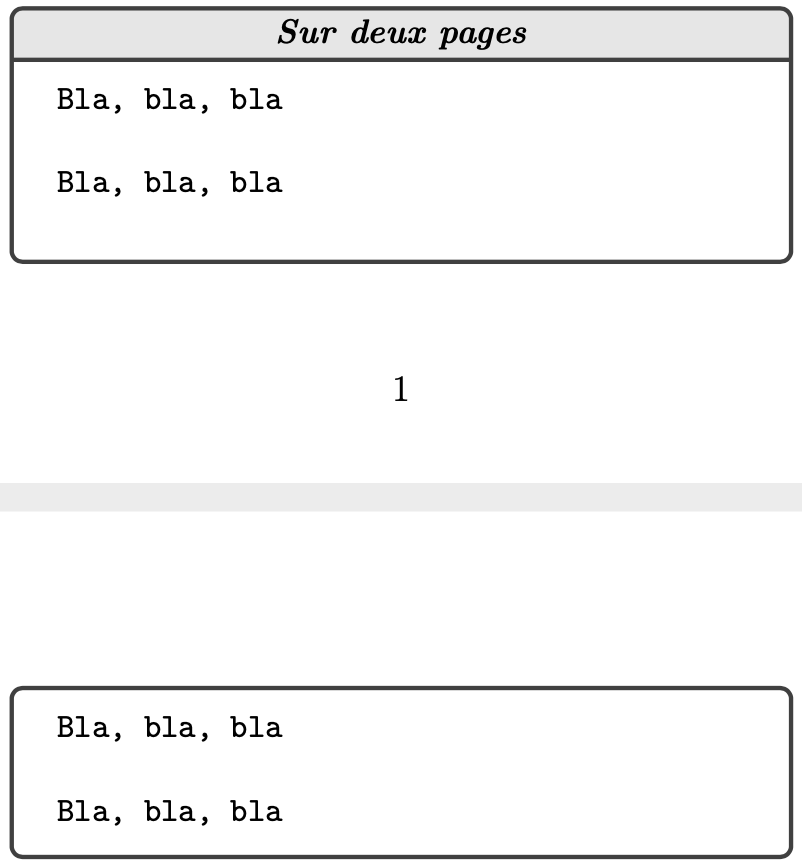
\includegraphics[scale = .5]{images/pseudo-verb-broken[fr].png}}
\end{figure}


% ---------------------- %
\newpage

\section{Historique}

Nous ne donnons ici qu'un très bref historique récent
\footnote{
	On ne va pas au-delà de un an depuis la dernière version.
}
de \verb+tnspverb+ à destination de l'utilisateur principalement.
Tous les changements sont disponibles uniquement en anglais dans le dossier \verb+change-log+ : voir le code source de \verb+tnspverb+ sur \verb+github+.

\begin{description}
% Changes shown - START

    \medskip
    \item[2020-09-06] Première version \verb+0.0.0-beta+.

% ------------------------ %

% Changes shown - END 
\end{description}


\newpage
\section{Toutes les fiches techniques} \label{techincal-ids}









\subsection{Écriture \texttt{pseudo verbatim}}



\IDenv[o]{pseudoverb}{1}

\IDoption{} on utilise un système clé/valeur.
\begin{enumerate}
	\item \verb#title# est le titre du cadre.
	      Par défaut \verb#title = {}#.

	\item \verb#frame# demande d'ajouter un cadre.

	\item \verb#center# sert à centrer le contenu.

	\item \verb#width# donne le coefficient multiplicatif à appliquer à la largeur de la ligne.
	      Par défaut \verb#width = 1#.
\end{enumerate}




\end{document}
